\section{Introduction}
\label{sec:intro}

BGP Monitor (BGPmon) is a light-weight, scalable,  and extensible system for monitoring BGP routing.
BGPmon collects routing data by imitating a real BGP router and peering with other BGP routers.
All routing updates received from the peers are converted into a convenient XML format and output to interested clients.
In addition, BGPmon can output periodic routing tables and control messages.
BGPmon can also label routing data to simplify later analysis.   

BGPmon clients receive the data from one or more BGPmon instances and perform a variety of data parsing tasks.
Any program that can establish a TCP connection and parse XML can become a client.
Some clients archive updates to disk,  other clients identify and forward only updates that meet some criteria, and so forth.
%A number of BGPmon clients are provided as part of the base distribution.    

\subsection{Audience}

This document is intended for readers interested in installing, configuring, and using BGPmon.
Readers interested in the underlying design philosophy of the BGPmon system should refer to the technical paper\cite{imc08}.
Readers interested in understanding the implementation details of BGPmon or modifying the source code should refer to the detailed technical specification found in \cite{massey08tech}.     

\subsection{BGPmon Design Overview}

The BGPmon design extends the scalable event driven architecture in \cite{seda} to meet the requirements of BGP monitoring.
BGPmon is a stream based monitoring system; an architectural overview is shown in Figure \ref{fig:arch}.
BGPmon receives BGP messages from peer routers, performs some optional labeling, converts the data to an XML format, and passes the resulting data to clients via TCP connections.
BGPmon clients receive an event stream in real-time from peer routers. 
It is also possible to read historical event streams from archival sources, for example, an archival source could be obtained from RouteViews.
%The single stream incorporates both incremental BGP update messages and periodic routing table snapshots.
BGPmon uses XML to provide easy extensibility, integrate with common tools, and allow local data annotations.      

\begin{figure}[hbt]
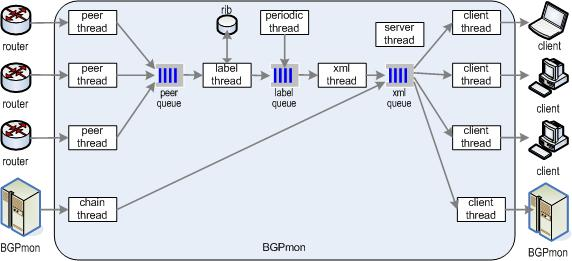
\includegraphics[width=.9\textwidth]{figs/architecture.png}
\caption{\label{fig:arch}An overview of the BGPmon architecture.}
\end{figure}

\subsubsection{Peers}
BGPmon collects BGP updates by establishing peering sessions with routers.
BGPmon emulates the behavior of a peering router, but only listens; BGPmon does not implement any routing polices, perform any route selection, manage forwarding tables, or forward packets.
The BGPmon design allocates one thread for each peering session.
All messages received from a peer are written into the Peer queue for processing by later modules.

\subsubsection{Labeling}
In the BGPmon design, nearly all data processing is assumed to occur at the clients.
However, BGPmon can be configured to add labels to each update received from a BGP peer router.
The labels produced by BGPmon include: \\

\begin{table*}[h!]
\centering{
\begin{tabular} {| l | l |}
\hline
\emph{NANN} &	a New ANNouncement (prefix not previously reachable) \\
\hline
\emph{DPATH}	&  an update announcing a Different AS PATH\\
\hline
\emph{SPATH}	&  an update announcing the Same AS PATH, but some other change\\ 
\hline
\emph{DANN} &	a Duplicate ANNouncement (no change in any attribute)\\
\hline
\emph{WITH} & a WITHdraw (prefix no longer reachable)\\
\hline
\emph{DWITH} &	a Duplicate WITHdraw (unreachable prefix withdrawn)\\
\hline
\end{tabular}
\caption{\label{tbl:intro:labels}The labels assigned to updates by BGPmon.}
}
\end{table*}

Calculating the labels requires BGPmon to store RIB\_IN tables from each peer. 
Storing RIB\_IN tables can consume substantial amounts of memory and add some computational costs. 
Therefore, RIB\_IN tables can be disabled on a per-peer basis, but labeling is not possible if RIB\_IN tables are disabled.
Labeling is discussed further in Section \ref{sec:configure:peers:configureparameters}.

\subsubsection{Chains}

A single BGPmon instance can typically handle a large number of peers and clients.
However, it may be useful to run multiple instances of BGPmon and connect them together into a single chain.
Data from one BGPmon can be fed into a second BGPmon instance.
Clients are oblivious to chains and, to the client,  it appears as though all data is being collected by a single BGPmon instance.
BGPmon chains provide a range of powerful options for scaling to vast numbers of peers, adding additional robustness, or separating peering and collector functions.

As an example, suppose an administrator in Denver wanted to monitor BGP routers at exchange points in Los Angeles and London.    A single BGPmon instance running in Denver could peer with routers at both the Los Angeles and London exchange points.   However, this requires the use of multi-hop BGP and if the BGPmon instance fails, all data is lost.    An alternate strategy would be to deploy a BGPmon instance in London and second BGPmon instance in Los Angeles.     The London and Los Angeles BGPmon instances could chain to a third BGPmon instance in Denver.    The LA and London BGPmon instances feed data to the Denver instance which in turns provides data to clients.    Clients are unaware if the data received comes from a single instance or chain of BGPmons.     Section \ref{sec:configure:chains} describes how to configure BGPmon chains. 


\subsubsection{Clients}
The BGPmon server is designed to simply collect, aggregate and report data; BGPmon itself does not archive data or perform complex analysis on it.
These tasks are reserved for BGPmon clients.
A client receives XML data from BGPmon via a TCP connection and then performs the desired data processing tasks.
Users can build their own clients to suit their individual needs.
%A small number of sample clients and common used clients are included in the BGPmon distribution.   Clients provided in the base distribution include:

%\begin{itemize}

%\item{\emph{BGP Data Archive Client:}   logs the updates received from BGPmon to disk and also periodically writes routing tables (RIB\_INs) to disk.    }
%
%\item{\emph{BGP Data Statistics Client:}   creates and maintains HTML pages that track the status of BGPmon.  The results can be displayed on a website to provide on-line tracing of BGPmon behavior.}
%
%\item{\emph{BGP Data Real-Time Filter:}   receives updates from BGPmon and passes only the updates matching a configured criteria to downstream clients.    This allows users to select a set of interesting updates from the potentially vast volume of messages sent by BGPmon.}
%
%\item{\emph{BGP Sample Client:}  receives updates from BGPmon and acts as starting point for designing and implementing additional site-specific clients.  }
%
%\end{itemize}

\subsection{BGPmon Configuration}

BGPmon is designed to imitate a router, and its configuration is similar to that of major router vendors.   An administrator logs into BGPmon and, after passing authentication checks,  has access to the administrative portion of BGPmon.   Similar to the BGP routers sold by large vendors,  there are two access levels.    Initially, an administrator is connected in \emph{access mode}.   Access mode allows the administrator to view statistics, show routing tables, and generally view (but not change) configuration parameters.    BGPmon may be configured to allow arbitrary users to login and display statistics,  similar to what a user could do if granted access to a router at an ISP.    

In order to change the configuration,  the user must switch to \emph{enable mode}.   An administrator that has entered \emph{enable mode} can perform all BGPmon configuration actions such as adding, deleting, or modifying BGP peers,  disabling clients, setting access control policies, and so forth.    All changes are stored in memory and will be lost if BGPmon restarts.   At any time, an administrator in \emph{enable mode} can save the current BGPmon configuration to a file.      The configuration file can then be loaded in subsequent restarts.    

If no configuration file is specified at boot time,  BGPmon attempts to load a default configuration file.    If no configuration is specified and no default configuration file is found,  BGPmon allows the administrator to login on port 50000.   An alternate default port number can also be specified as a command line parameter to BGPmon.

%\subsection{Organization of This Document}
%
%Section \ref{sec:install} describes how to install the base BGPmon software and describes the resource requirements for BGPmon.
%Section \ref{sec:cli} describes how to login and modify the BGPmon configuration.
%Section \ref{sec:label} describes the BGPmon labeling options.
%Section \ref{sec:chains} describes how to configure multiple BGPmon instances into a chain.
%Section \ref{sec:clients} describes BGP Monitor clients, including both standard clients included in the base package and guidelines for building new clients.
%Section \ref{sec:trouble} provides troubleshooting help and Section \ref{sec:ack} acknowledges the many people and organizations that helped develop BGP Monitor.    
%Appendix \ref{sec:cliref} describes the full set of commands available to BGPmon administrators.
